\likechapter{Введение}

    Интернет вещей (IoT) объединяет устройства в компьютерную сеть и позволяет им собирать, анализировать, обрабатывать и передавать данные другим объектам через программное обеспечение, приложения или технические устройства.

    
    Цель проекта <<Mini Cooper 2.0>> состоит в реализации системы устройств, которые способны передавать информацию о состоянии автомобиля в реальном времени.
    
    Машина состоит из следующих датчиков: два термометра (внутренний, для измерения температуры в салоне, и внешний, для измерения температуры за бортом автомобиля), спидометр, четыре датчика давления (по одному на каждую шину) и датчик GPS, для передачи координат о местонахождении.
    
    
    \begin{figure}[!ht]
		\centering
		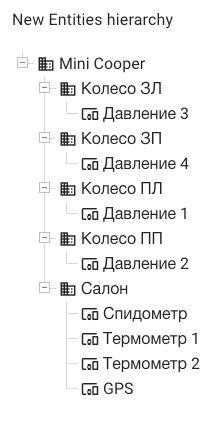
\includegraphics[scale=0.8]{pictures/5.jpg}
		\caption{Иерархия автомобиля}
		\label{fig1}
	\end{figure}